
\subsection{Mission Study and Management Plan  }
\label{sec:management}

\vspace{-0.05in}

\subsubsection{Study Plan}

\vspace{-0.05in}

The mission study is open to the entire CMB community and includes more than 50 scientists. 
To gain maximum benefit from \planck , LiteBIRD, and CORE we invited international members to participate. 
The work is organized into Working Groups (WG) that represent each of the main themes of the study; see 
Figure~\ref{fig:management}. Working groups are led by members of the study's Executive Committee, 
as listed in the Figure. Although Figure~\ref{fig:management} suggests distinct boundaries between the 
WGs we expect and encourage significant overlap and feedback. It is not practical to enumerate all 
the interdependencies. 

%and as outlined in more detail below? 
%NASA/JPL, lead by CoI Lawrence (Chief Scientist 
%at JPL and US \planck\ team lead), will assist with mission design. The PI will lead the study of the Imager and will interface with 
%the JPL team. Al Kogut (PI of the Explorer-proposed PIXIE) will lead the spectrometer study. Knox and Flauger will lead the theory and 
%foregrounds aspects of the study; McMahon and Lee (PI of the US LiteBIRD team) will lead the study of relevant technologies.  

\begin{figure}[ht!]
\hspace{-0.1in}
\parbox{3.5in}{\centerline {
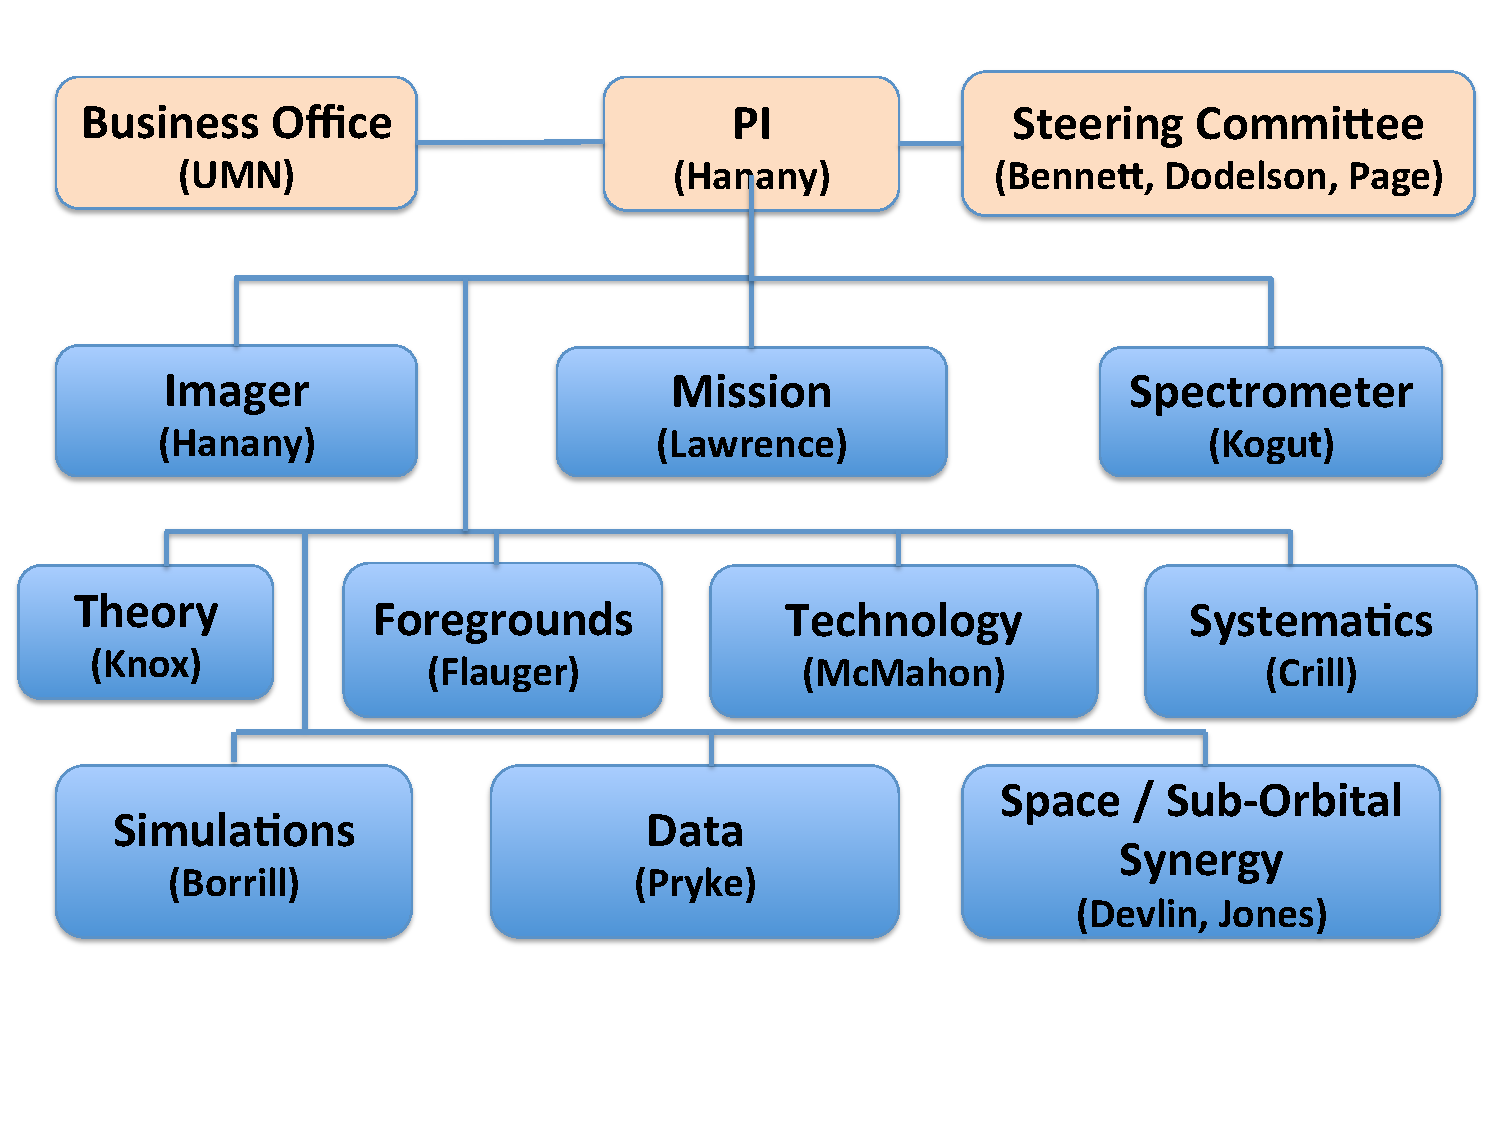
\includegraphics[width=3.5in]{Figures/OrgChart_names_noEC} } }
\hspace{0.05in}
%\end{center}
\parbox{2.8in}{
\caption{ \small \setlength{\baselineskip}{0.95\baselineskip}
Management structure of the CMB Probe. A steering committee advises the PI. The study is led by the PI 
through an Executive Committee. Each member of the committee is in charge of a specific Working Group (blue boxes). Significant overlap and feedback is expected between the working groups.  Participation in the Working Groups is open to all members of the CMB community. 
\label{fig:management} } }
\vspace{-0.1in}
\end{figure}

The study will be carried out through intra- and inter-WG teleconferences; mission design teleconference with JPL engineers; 
mission design meetings at JPL; and a community workshop that is described in more detail below under the `Space / Sub-Orbital 
Synergy' WG.  We now describe the planned work for each of the WG. 

$\bullet$ {\bf Theory (Knox)} \hspace{0.1in} This WG will survey, summarize, and prioritize the set of 
science goals for the Probe.  Given input on target frequency bands, assumptions about foregrounds, 
instrument systematics, and instrument noise levels the group will generate forecasts for the impact of 
the Probe�s products and their ultimate significance for physics and astrophysics. This group 
will also investigate how to optimally combine and cross-correlate the Probe's data with other 
data sets. This is an area of strong overlap with the Data WG. 

$\bullet$ {\bf Mission (Hanany) and connection with JPL (Lawrence)} \hspace{0.1in} The Mission WG is responsible 
for defining the overall mission architecture including telescope implementation, cooling, telemetry, mass, 
power, and cost. The WG will work closely with the JPL lead scientist (Lawrence) and JPL mission engineers. 

$\bullet$ {\bf Imager (Hanany) and Spectrometer (Kogut)} \hspace{0.1in} The imager and spectrometer WGs will 
translate the science goals to 
mission requirements and to a set of optional designs. The designs will include telescopes of various configurations, 
focal planes with several candidate detector technologies and readout schemes, optical 
elements, and cooling strategies. These groups will similarly consider 
the options for spectrometers.  Both groups will interact frequency and work closely 
with the Mission WG and with the JPL team to assess the relative merits 
of the designs. We will consider an imager-only design, a spectrometer-only design, and
a combined instrument.  

$\bullet$ {\bf Technology ( )} \hspace{0.1in}

$\bullet$ {\bf Space / Sub-Orbital Synergy (Devlin, Jones)} \hspace{0.1in} By the time the \ac{CMB} probe is likely to fly,
significant advances will have been made on the ground. This is true regardless of the state of the proposed CMB-S4
effort, and even more so should funding for S4 becomes available soon. This WG will assess and recommend the 
most appropriate design parameters such that the data sets from the Probe and sub-orbital measurements complement each other. 
Pertinent questions include: to what extent should the aperture size of the Imaging Probe rely on delensing capabilities provided by 
high resolution measurements from the ground? What is the optimal resolution of a space-based mission from the point 
of view of providing foreground subtraction capabilities to sub-orbital missions? What is an optimal overlap in $\ell$-space
coverage? Does the design of a spectrometer depend on the specifics of data available from sub-orbital measurements? 

We are planning a community workshop to address these question, including forming a community consensus on the 
question of the need for a space mission if CMB-S4 is funded. 

$\bullet$ {\bf Data Analysis and Exploitation (Pryke)} \hspace{0.1in}
The full sky nature, the broad frequency coverage, and the high 
sensitivity of the CMB-Probe will generate a legacy
data set surpassing that of \planck. This working group will plan for 
the extraction of cosmological and astrophysical
products from the Probe's data. This includes exploring component 
separation techniques and the resulting core science analysis performance,
as well as exploring synergies with sub-orbital measurements at
CMB frequencies and cross-correlations with orbital and
sub-orbital data at other wavelengths. It will assess whether specific 
synergies suggest preferring
some mission parameter values over others. Examples include adjusting 
the resolution, and frequency coverage.
%The group will also survey possible sources of systematic uncertainties that are introduced during 
%the analysis process and how these can be addressed during mission 
%design, implementation, and data analysis. 

$\bullet$ {\bf Systematics (Crill)} \hspace{0.1in} We plan to build an end-to-end simulation pipeline that will 
generate simulated measurements at an instrumental level, and feed them into the notional analysis pipeline, 
including foreground/CMB component separation and power spectral analysis.  With this simulation pipeline 
we will explore mitigation of systematic errors by design, for example implementing modulation 
schemes and modulator technologies, and mitigation of systematic errors by analysis techniques.  
This pipeline will be used to define requirements for a notional mission, and would be helpful in 
prioritizing the Probe's technology development needs. 
%\comred{add more from the systematics section?}

% To incorporate instrument systematics due to beams, bandpass mismatches, correlated noise, etc., time domain based simulations will be required.

$\bullet$ {\bf Foregrounds (Flauger) } \hspace{0.1in} High fidelity measurement and subtraction of foregrounds will 
permeate all aspects of the study plan. We will construct foregrounds models that encompass all the known emission 
complexities. The models will be informed by physically motivated inputs~\cite{Bruce+Fraisse2009,Hensley_etal} 
and measured data including, for example the spatial variations and departures from a single spectral index 
emission law for galactic dust~\cite{Planck2015-X;Planck2015-L;Planck2015-XXIX;Boulanger2016}. 
The models will become inputs for the process of instrument optimization and for exercises in foreground subtraction. 
During instrument optimization 
we will assess an optimal selection for the number of frequency bands, their central frequencies and bandwidths, all 
subject to the constraint of finite focal plane area. This optimization is also informed by choices of detector technology. 
To carry out exercises in foreground subtraction, we will implement a simulation pipeline that will test the efficacy 
of different component separation methods including Commander, SMICA, SEVEM and NILC, which have been 
used with the \planck\ data~\cite{Planck2015-IX}. We will extract cosmological and astrophysical information 
from the component maps and their power spectra, and compare to the input values to assess the residual 
errors. During this stage too, we will benefit from the experience of the \planck\ data including its use 
of specific power spectral and parameter estimation approaches (e.g. Master~\cite{}, XFaster~\cite{}, and CosmoMC~\cite{}). 

$\bullet$ {\bf Simulations (Borrill)} \hspace{0.1in}



\vspace{-0.18in}

\subsubsection{Study Team}

\vspace{-0.05in}

The study consists of more than 50 scientists representing 
hundreds of years of experience with CMB theory, data analysis, and measurements on all platforms including satellite missions
that have already flown (WMAP, and \planck ) and the two proposed (LiteBIRD and CORE). 
The PI Hanany, who has more 
than 20 years of CMB ballooning experience, co-led MAXIMA and Archeops, was the PI of MAXIPOL and EBEX, and 
is a member of CORE's Executive Board, will have ultimate responsibility for the study. He 
is advised by a Steering Committee -- Bennett (Johns Hopkins), Dodelson (Chicago), and Page (Princeton) -- 
and assisted by a business office at the University 
of Minnesota.  An Executive Committee (EC) is in charge of the daily operation of the collaboration. The members
of the Steering and Executive Committees led and are leading operating CMB experiments that have 
produced the most compelling CMB 
polarization results. They include leaders and members of the WMAP, US \planck , US 
LiteBIRD, and US CORE teams. They include initiators and implementors of new millimeter-wave 
technologies, and of recognized experts in data analysis and theory. 

\comred{to be completed}

%Fisher

%OVERVIEW of PLAN


%INSTRUMENTAL PARAMETERS:

%FG MODELLING:
% Planck Sky Model, PSM \ref{}, and/or  Python Sky model, PySm \ref{}, 


%TECHNIQUES:
% CMB4cast (http://portal.nersc.gov/project/mp107/index.html)). 

%SIMULATIONS
%For a more in depth analysis, that can also probe biases in the parameters, we will simulate maps of the CMB and Foreground emission at each frequency with CAMB and PSM (or PYSM) packages respectively and HEALpix modules \ref{}. Noise simulations will then be added to the signal maps. While white noise or anisotropic noise are straightforwardly simulated directly on map domain, 1/f or correlated noise requires simulating time ordered data according to a noise prescription or generator (eg akin to LevelS \ref{} used in Planck). The convolution of the simulated maps with the Gaussian beams can be performed straightforwardly with HEALpix modules, while the convolution with more realistic beams is harder but can be performed with approaches such as FEBeCOP \ref{}, developed for Planck data analysis. To apply the latter an optical beam and scanning strategy needs to be specified and adopted by the software.

%The next step is to clean the frequency maps from foregrounds and generate the 'clean' CMB map, using techniques such as Commander, SMICA, SEVEM and possibly NILC \ref{Planck2015-IX}. This is followed by estimation of auto and cross-correlation angular power spectra of the maps using say Master based \ref{}  or XFaster \ref{} based techniques and propagated to parameter estimation using CosmoMC or Multinest sampling. Along with this standard procedure we will also apply a novel technique based on direct Bayesian MCMC inference of cosmological parameters in the presence of foregrounds, without resorting to Likelihood approximations (an extension of the method presented in  \ref{Jewelletal2016}). 
%The latter will be integrated with Commander, allowing to bypass the angular power spectrum estimation as it samples Cosmological and Foregrounds parameters directly from the simulated maps. As in this approach the foreground parameter fits (including the spectral index) is performed pixel by pixel, the spatial variation of the spectral index is naturally accounted for. 

%As mentioned earlier 1/f or correlated noise requires simulating time ordered data. To analyse the resulting maps another ingredient is needed, the pixel-to-pixel noise correlation matrix. For a large number of pixels the estimation of this matrix is computationally intensive. As 1/f and correlated noise leaves mostly in the large angular scales and we resort to studying these effects on low resolution maps (reducing computational costs), hybridized with higher resolution maps for the white noise component. 

%It should be stressed that to fully assess the performance of a given instrument design, in view of both foreground residuals and the presence of systematics, realistic simulations are essential. These include time domain based simulations which can be generated using HPC4CMB ((https://github.com/hpc4cmb)) based on TOAST 
%(data framework, including on-the-fly simulation capabilities with full detector beam, bandpass and noise properties)), 
%and a destriper based map-making algorithm such as libMADAM. 


%FOM
%Finally to quantify performance we will need to define a figure of merit, FOM. Examples of possible FOM, are: the effective noise in the I,Q,U maps after foreground cleaning (effectively quantifying the noise degradation due to the presence of residual foregrounds); uncertainty and biases in the parameters; the evidence of the best fit model for each instrumental design (used as a qualifier of the instrumental design itself), etc.

